\documentclass[11pt]{article}

\usepackage[margin=1in]{geometry}
\usepackage{booktabs}
\usepackage{graphicx}
\usepackage{hyperref}
\usepackage{siunitx}
\usepackage{caption}
\usepackage{subcaption}

\title{Information Retrieval Final Assignment\\Cross-Encoder Re-ranking, Fusion, and Query Expansion}
\author{\textbf{Student:} Mayuresh Khalane \\\textbf{Course:} Information Retrieval}
\date{\today}

\begin{document}
\maketitle

\section{Experimental Setup}
We fine-tuned three cross-encoder re-rankers on the MSMARCO passage re-ranking dataset for approximately one hour each, following the provided assignment notebooks. We then evaluated the fine-tuned checkpoints on the 43 TREC Deep Learning (DL) 2019 queries using the official top-1000 candidate set and report NDCG@10, Recall@100, and MAP@1000.

\paragraph{Models.}
\begin{itemize}
  \item \texttt{cross-encoder/ms-marco-MiniLM-L-2-v2}
  \item \texttt{cross-encoder/ms-marco-TinyBERT-L-2-v2}
  \item \texttt{distilroberta-base}
\end{itemize}

\paragraph{Metrics.} We report NDCG@10, Recall@100, and MAP@1000 on TREC DL'19.

\section{Task 1: Fine-tuning and Evaluation Results}
Table~\ref{tab:task1} shows the evaluation results for the three fine-tuned models. The ``Steps'' column reports the last observed training step around the one-hour mark (as requested in the assignment).

\begin{table}[t]
\centering
\small
\sisetup{round-mode=places,round-precision=4}
\begin{tabular}{l r S S S}
\toprule
Model & Steps ($\approx$1h) & {NDCG@10} & {Recall@100} & {MAP@1000} \\
\midrule
MiniLM-L-2-v2      & 35000 & 0.6721 & 0.4988 & 0.4339 \\
TinyBERT-L-2-v2    & 95000 & 0.6917 & 0.5052 & 0.4553 \\
DistilRoBERTa-base & 11000 & 0.5463 & 0.4733 & 0.3968 \\
\bottomrule
\end{tabular}
\caption{Task 1 results on TREC DL'19 (43 queries) for the three fine-tuned cross-encoder re-rankers.}
\label{tab:task1}
\end{table}

\subsection{Discussion}
Overall, the TinyBERT-L-2-v2 checkpoint achieved the strongest effectiveness across all reported metrics, followed closely by MiniLM-L-2-v2. DistilRoBERTa underperformed the other two models on this test set.

A plausible explanation is that the MSMARCO-tuned MiniLM and TinyBERT checkpoints are already well-aligned with passage re-ranking, and fine-tuning further adapts them to the pairwise preference signal in MSMARCO. DistilRoBERTa starts from a general-purpose language model initialization, so for a fixed one-hour budget it may not converge as well as the already task-adapted MS MARCO cross-encoders.

Although TinyBERT is best here, this does not guarantee it will be best for all unseen queries. The differences between models can depend on query type, the candidate generation stage, and distributional shift between MSMARCO training data and TREC DL queries.

Finally, a practical limitation is efficiency: higher-capacity models typically provide better ranking signals but at greater latency. In real systems, the best choice depends on both effectiveness and computational constraints.

\begin{figure}[t]
\centering
\begin{subfigure}[b]{0.48\linewidth}
  \centering
  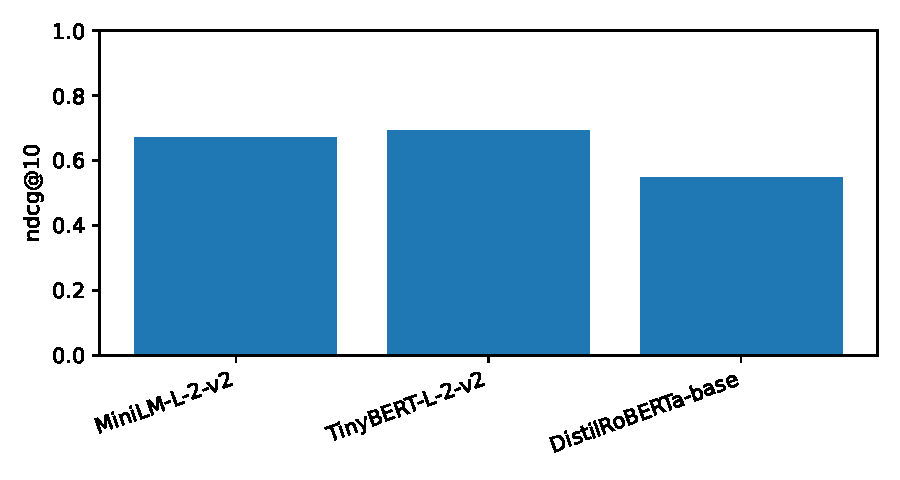
\includegraphics[width=\linewidth]{figures/task1_ndcg@10.pdf}
  \caption{NDCG@10}
\end{subfigure}
\hfill
\begin{subfigure}[b]{0.48\linewidth}
  \centering
  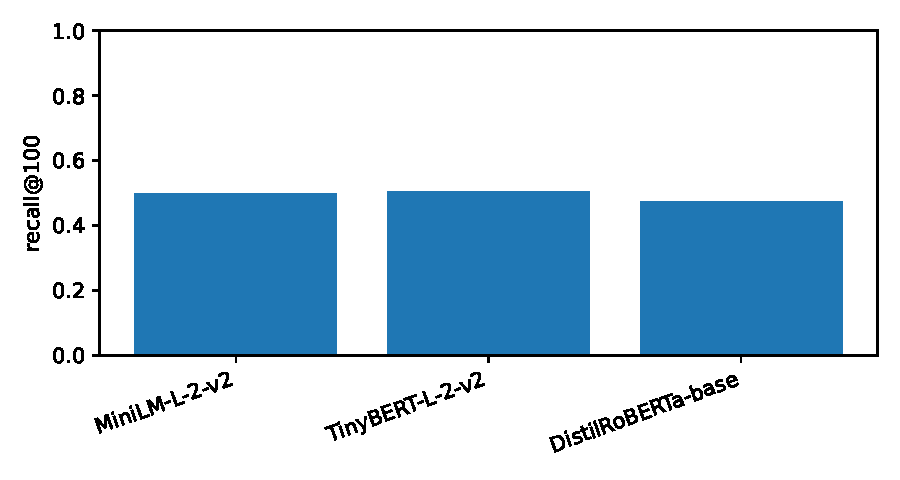
\includegraphics[width=\linewidth]{figures/task1_recall@100.pdf}
  \caption{Recall@100}
\end{subfigure}

\vspace{0.5em}
\begin{subfigure}[b]{0.48\linewidth}
  \centering
  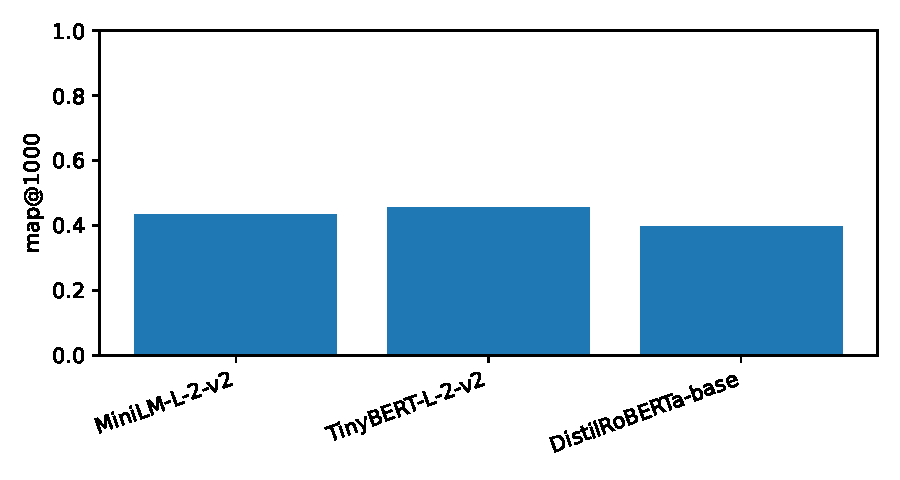
\includegraphics[width=\linewidth]{figures/task1_map@1000.pdf}
  \caption{MAP@1000}
\end{subfigure}
\hfill
\begin{subfigure}[b]{0.48\linewidth}
  \centering
  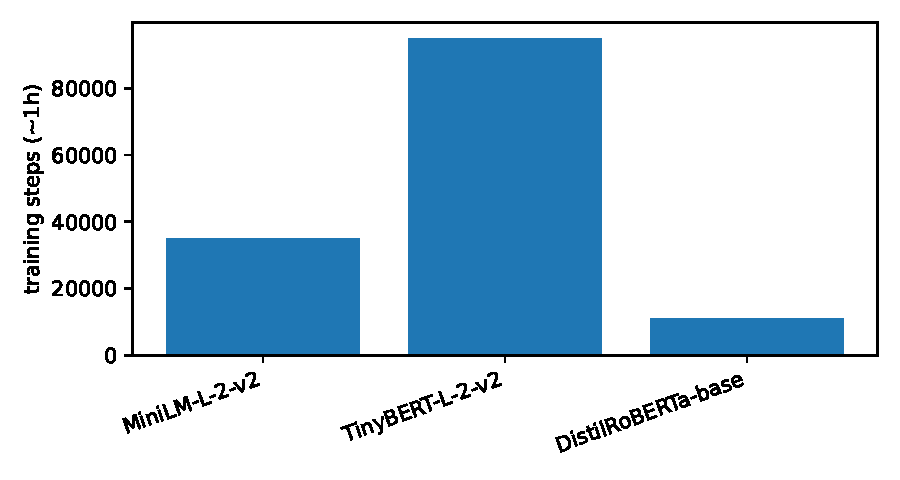
\includegraphics[width=\linewidth]{figures/task1_steps.pdf}
  \caption{Training steps ($\approx$1h)}
\end{subfigure}
\caption{Task 1 results summary.}
\label{fig:task1_plots}
\end{figure}

\section{Task 2 and 3: Fusion with ranx (Work Plan)}
We provide a fully script-based pipeline for Tasks 2 and 3 using \texttt{ranx}. Given the three TREC run files produced in Task 1, we can fuse the runs with five fusion methods (Task 2), then select the best fusion method and apply it to all 2-run combinations (Task 3).

\paragraph{Note.} In our workflow, these tasks are executed by \texttt{scripts/fuse\_and\_eval.py}. The resulting CSV tables can be directly included in the report.

\section{Task 4 and 5: Query Expansion (Work Plan)}
We provide scripts for LLM query expansion with and without pseudo-relevance feedback (PRF) based on the method described in the paper ``Query Expansion by Prompting Large Language Models''. We implement:
\begin{itemize}
  \item \textbf{Task 4:} Expansion via a chain-of-thought style prompt (\texttt{cot}).
  \item \textbf{Task 5:} Expansion with PRF context taken from top-ranked candidates (\texttt{cot\_prf}).
\end{itemize}

\section{Reproducibility}
All experiments are runnable as Python scripts (no notebooks required). The main entry points are:
\begin{itemize}
  \item Fine-tuning: \texttt{scripts/fine\_tune.py}
  \item Evaluation: \texttt{scripts/evaluate.py}
  \item Fusion: \texttt{scripts/fuse\_and\_eval.py}
  \item Query expansion experiments: \texttt{scripts/run\_query\_expansion\_experiments.py}
\end{itemize}

\end{document}
